% CVPR 2025 Paper Template; see https://github.com/cvpr-org/author-kit

\documentclass[10pt,twocolumn,letterpaper]{article}

%%%%%%%%% PAPER TYPE  - PLEASE UPDATE FOR FINAL VERSION
% \usepackage{cvpr}              % To produce the CAMERA-READY version
\usepackage[review]{cvpr}      % To produce the REVIEW version
% \usepackage[pagenumbers]{cvpr} % To force page numbers, e.g. for an arXiv version

% Import additional packages in the preamble file, before hyperref
%
% --- inline annotations
%
\newcommand{\red}[1]{{\color{red}#1}}
\newcommand{\todo}[1]{{\color{red}#1}}
\newcommand{\TODO}[1]{\textbf{\color{red}[TODO: #1]}}
% --- disable by uncommenting  
% \renewcommand{\TODO}[1]{}
% \renewcommand{\todo}[1]{#1}



% It is strongly recommended to use hyperref, especially for the review version.
% hyperref with option pagebackref eases the reviewers' job.
% Please disable hyperref *only* if you encounter grave issues, 
% e.g. with the file validation for the camera-ready version.
%
% If you comment hyperref and then uncomment it, you should delete *.aux before re-running LaTeX.
% (Or just hit 'q' on the first LaTeX run, let it finish, and you should be clear).
\definecolor{cvprblue}{rgb}{0.21,0.49,0.74}
\usepackage[pagebackref,breaklinks,colorlinks,allcolors=cvprblue]{hyperref}

%%%%%%%%% PAPER ID  - PLEASE UPDATE
\def\paperID{*****} % *** Enter the Paper ID here
\def\confName{CVPR}
\def\confYear{2025}

%%%%%%%%% TITLE - PLEASE UPDATE
\title{Plagiarism Precise Localization Based on FAISS and SentenceTransformer}

%%%%%%%%% AUTHORS - PLEASE UPDATE
\author{
    张三\\
    北京大学\\
    {\tt\small zhangsan@example.com}
    \and
    李四\\
    清华大学\\
    {\tt\small lisi@example.com}
}

\begin{document}
\maketitle
\begin{abstract}
This paper proposes a text plagiarism detection method based on FAISS and SentenceTransformer, aimed at improving the accuracy and efficiency of plagiarism detection. Our approach not only identifies plagiarism but also accurately pinpoints plagiarized sections, including direct quotations, paraphrasing, or disguised content. Experimental results demonstrate that this method performs well in terms of accuracy and efficiency on large-scale datasets, providing educational institutions with a more comprehensive tool for academic integrity detection, thereby contributing to the fairness and integrity of the academic environment.
\end{abstract}
\usepackage{enumitem}
\section{Introduction}
With the rapid development of large language models (LLMs) and retrieval tools in the field of natural language processing, their applications have gradually permeated the education and academic sectors, especially showing great potential in areas such as automated grading, personalized learning, and content generation. However, with the widespread application of these technologies, academic integrity issues have become increasingly complex and severe. Problems like assignment plagiarism, ghostwriting, and code plagiarism not only undermine the fairness of the academic environment but also present significant challenges for educational institutions in terms of management. Traditional plagiarism detection methods mainly rely on simple text matching or manual inspection, which, while effective in identifying explicit textual similarities, often fail to detect implicit plagiarism or modified plagiarized texts.

Currently, the academic community has begun to explore more advanced plagiarism detection methods, including semantic matching techniques based on large language models and retrieval-augmented frameworks. These methods offer deeper text understanding and can provide support in more complex plagiarism scenarios. However, most existing studies focus on determining the overall similarity between texts, and there is still a lack of effective solutions for precisely pinpointing specific plagiarized sections of the text. Therefore, in this paper, we propose an improved approach based on adjusting the parameters of FAISS~\cite{FAISS} and SentenceTransformer, aiming to enhance the accuracy and efficiency of plagiarism detection, especially in terms of accurately identifying and locating plagiarized segments.

FAISS (Facebook AI Similarity Search) is an efficient similarity search and clustering tool that can quickly process large-scale text data and identify content highly similar to the query text. In our research, we adjust the parameters of FAISS and SentenceTransformer to optimize the model's search and matching strategies, allowing us not only to detect whether Student A has plagiarized from Student B, but also to precisely highlight the specific plagiarized parts, such as direct quotes, rephrasing, or simply changing certain names.

This improved approach, based on large-scale data and deep learning technology, can address the limitations of traditional plagiarism detection methods in terms of accuracy and efficiency, providing educational institutions with a more comprehensive and precise plagiarism detection tool. By combining automated model judgment with subsequent manual review, we can more efficiently address complex academic integrity issues and provide technical support to maintain fairness and integrity in the academic environment.

There are some of our main contributions:

\begin{enumerate}
    \item \textbf{Classify plagiarized texts}:  
    We successfully utilized FAISS to classify plagiarized texts into three categories:  
    \begin{itemize}
        \item \textbf{Non-plagiarized text}: Non-plagiarized text refers to cases where the similarity between Text A and Text B is relatively low, generally indicating no plagiarism.  
        \item \textbf{Explicitly plagiarized text}: Explicitly plagiarized text refers to cases where the similarity between two texts is extremely high, such as when only proper nouns are changed or numbers are slightly adjusted.  
        \item \textbf{Implicitly plagiarized text}: Implicitly plagiarized text refers to cases where the similarity between two texts is lower, but plagiarism may still exist. A simple example is plagiarism achieved by merely changing the order of sentences.  
    \end{itemize}

    \item \textbf{Proposed a visualization algorithm for plagiarized text}:  
    We developed a simple yet effective method to highlight plagiarized content. Experiments have demonstrated that this algorithm performs well in practice.  

    \item \textbf{Our model}:  
    We built a simple demo that allows users to get a general idea of the model’s performance before using the complete version.
\end{enumerate}



\section{Related work}

\subsection{GPT-4o}
\ 

GPT-4o and GPT-4o \cite{chatgpt}Mini are advanced natural language processing models provided by OpenAI, offering powerful capabilities in text comprehension and generation. They can efficiently handle complex tasks such as text generation, language translation, and conversation. These models \cite{yuanjibao} emphasize the generally low quality of existing plagiarism text datasets, which are characterized by uneven data distribution, limited corpus size, and a lack of diversity in plagiarized texts. These challenges not only constrain the training effectiveness of plagiarism detection models but also limit their ability to handle complex plagiarism scenarios. To address these issues, this study utilizes GPT-4 to generate three types of data: non-plagiarized texts, implicit plagiarism texts, and explicit plagiarism texts. This generation strategy, by simulating various types of plagiarism behaviors, significantly enhances the diversity and quality of the dataset.

\subsection{FIASS}
\

FAISS is an open-source library developed by Facebook, specializing in fast and efficient similarity search and clustering. It is particularly well-suited for handling large dense vector datasets, such as text or image features extracted from deep learning models. In text similarity tasks, FAISS offers various indexing algorithms (such as inner product and Euclidean distance) and supports GPU acceleration, significantly improving search efficiency.

\subsection{SentenceTransformer}
\

SentenceTransformer is a Python library designed for converting sentences or paragraphs into embedding vectors, based on the Transformer architecture. By utilizing pre-trained models (such as BERT, RoBERTa, or MPNet), it generates semantically rich vector representations, facilitating subsequent similarity computations or clustering analyses.

\subsection{NLTK}
\

NLTK tokenizer is part of the Python natural language processing library NLTK (Natural Language Toolkit), used to split text into smaller units such as words or sentences. It provides a variety of efficient tokenization tools suitable for word tokenization, sentence tokenization, and other applications. The simplicity, ease of use, and high accuracy of the NLTK tokenizer make it an indispensable tool in text preprocessing, especially in fields such as natural language processing, information retrieval, and machine learning.
\section{Data description}
Our data comes from GPT-4o, GPT-4o mini, and some manually created data, all of which are text data. The data is divided into three categories: non-plagiarized text data, explicitly plagiarized text data, and implicitly plagiarized text data. Each category contains between 100 and 500 sentences, and they are further divided into original text data and test text data, with each original text data corresponding to a segment of test text data. For simplicity and ease of code implementation, each text segment contains no more than four sentences. Experiments have shown that this scale of data is sufficient to meet the basic requirements for plagiarism detection.
\usepackage{pgfplots}
\usepackage{graphicx}
\usepackage{amsmath}


\section{Method}

\subsection{Similarity Judgment Criteria}

\begin{figure}[h]
    \centering
    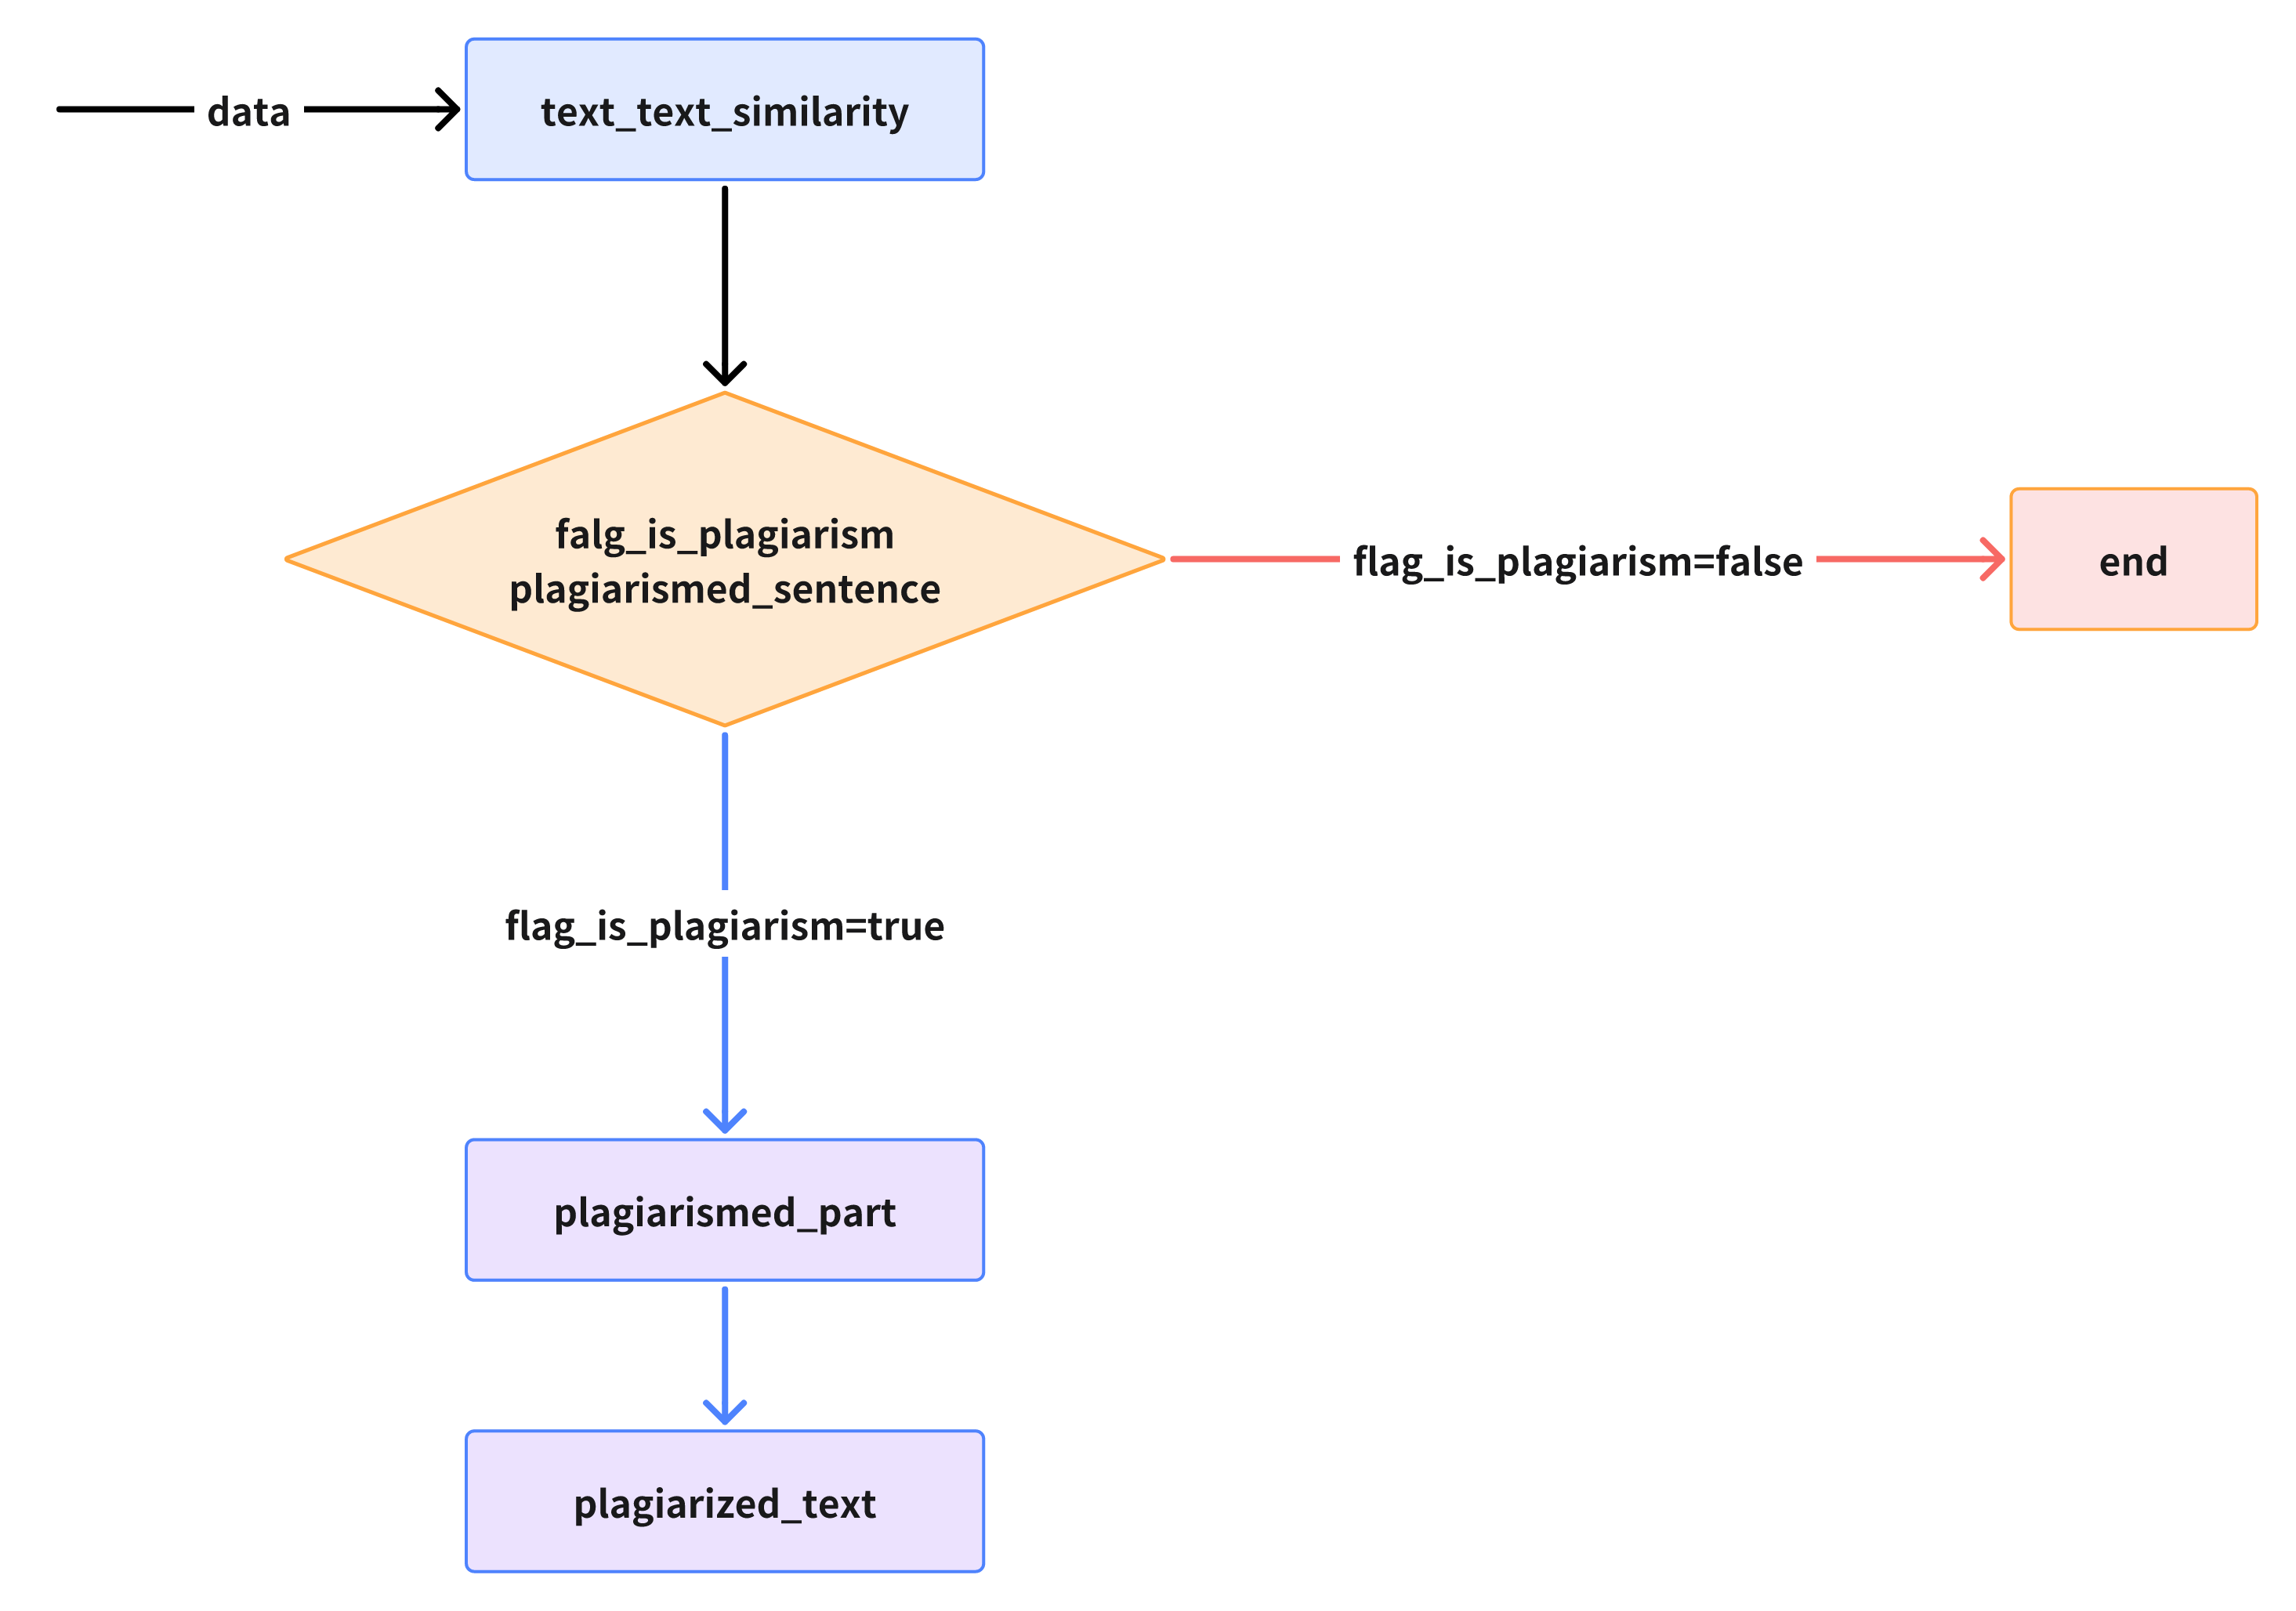
\includegraphics[width=1\linewidth]{png/system_demo.png}
    \caption{system framework}
    \label{fig:1}
\end{figure}

\subsubsection{Dot Product Similarity}
Dot Product Similarity is a common method for measuring the similarity between two vectors, especially in high-dimensional vector spaces. It calculates the similarity by computing the dot product (inner product) of two vectors.

Specifically, for two vectors \( A = (a_1, a_2, \dots, a_n) \) and \( B = (b_1, b_2, \dots, b_n) \), their dot product similarity is defined as:

\[
\text{Similarity}(A, B) = \sum_{i=1}^{n} a_i \cdot b_i
\]

In text processing or Natural Language Processing (NLP), vectors typically represent embeddings of words, sentences, or documents. By calculating the dot product of these embeddings, one can reflect the similarity between them. If the dot product of two vectors is large, it indicates that they are more similar in some feature space, meaning their similarity is higher.

\subsubsection{Cosine Similarity}
Cosine Similarity is a method for measuring the similarity of two vectors in terms of their direction, widely used in fields like text analysis and information retrieval. It determines the similarity between two vectors by calculating the cosine of the angle between them, without considering their magnitude.

Specifically, for two vectors \( A = (a_1, a_2, \dots, a_n) \) and \( B = (b_1, b_2, \dots, b_n) \), the cosine similarity is defined as:

\[
\text{Cosine Similarity}(A, B) = \frac{A \cdot B}{\|A\| \|B\|}
\]

where:
- \( A \cdot B \) is the dot product of vectors \( A \) and \( B \),
- \( \|A\| \) and \( \|B\| \) are the magnitudes (or lengths) of vectors \( A \) and \( B \), calculated as: 
  \[
  \|A\| = \sqrt{a_1^2 + a_2^2 + \dots + a_n^2}
  \]
  \[
  \|B\| = \sqrt{b_1^2 + b_2^2 + \dots + b_n^2}
  \]

The cosine similarity value ranges from -1 to 1:
\begin{itemize}
    \item \textbf{When the cosine similarity is 1}: It indicates that the directions of the two vectors are exactly the same.
    \item \textbf{When the cosine similarity is 0}: It indicates that the vectors are perpendicular and have completely different directions.
    \item \textbf{When the cosine similarity is -1}: It indicates that the directions of the two vectors are exactly opposite.
\end{itemize}

\subsubsection{Our Similarity Judgment Criteria}
\

During the experiment, we attempted to use two different similarity measures, but the performance of the dot product similarity was consistently poorer. This could be because the dot product similarity is sensitive to the position. In text plagiarism detection, the relative position is always crucial. A simple example is that the similarity between "This is an apple" and "An apple this is" should be high, but in dot product similarity, the similarity between these two sentences is not as high. Therefore, in this experiment, we used cosine similarity as our similarity measure.
\

We randomly generated 100 sentences similar to "This is an apple" and "An apple this is", and used two similarity evaluation methods to determine the accuracy of plagiarism detection. The results are as follows.
\[
\begin{array}{c|c}
\text{Method} & \text{Accuracy} \\
\hline
\text{Dot Product Similarity} & 74.48\% \\
\text{Cosine Similarity} & 85.69\% \\
\end{array}
\]

\subsection{Similarity evaluation}
\

Similarity evaluation is carried out based on the following three steps:
\subsubsection{Text Vectorization:}
\

The SentenceTransformer model, which is based on the Transformer architecture, is used here. SentenceTransformer focuses on mapping sentences or paragraphs to embedding vectors. Each sentence is transformed into a fixed-size high-dimensional vector, where each element of the vector represents different features or semantic information of the text. The position of the sentence in the high-dimensional space ensures that semantically similar sentences are closer to each other, while sentences with more semantic differences are farther apart. By doing this, different sentences or text segments are mapped to vector space, and we then compare these vectors to assess their similarity.

\subsubsection{Normalization:}
\

For each text's embedding vector, we apply the following formula for normalization:  
\[
\text{normalized\_embeddings} = \frac{\text{embeddings}}{\|\text{embeddings}\|}
\]  
The normalized embedding vectors have a length of 1, so during subsequent calculations, we focus only on the direction of the vector. Therefore, the similarity between texts is determined by their position in semantic space, independent of the length or complexity of the text itself.

\subsubsection{Similarity Calculation (Cosine Similarity):}
\

In a scenario with multiple texts, how can we identify the parts between two texts that are most likely plagiarized? To address this issue, we propose a simple yet effective method: splitting sentences. Since we can already retrieve plagiarism information between individual texts and provide a reliable quantitative metric, breaking a large problem into smaller, simpler sub-problems is always an effective approach. Specifically, the text is split into multiple sentences, and then each sentence is traversed individually. The two sentences with the highest similarity are considered the most likely plagiarized sentences. This method has the following advantages:

\subsection{Get the plagiarismed part}
\

In a scenario with multiple texts, how can we distinguish the most likely plagiarized parts between two texts? To address this issue, we propose a simple yet effective method: splitting sentences. Since we can already retrieve plagiarism information between individual texts and provide a reliable quantitative metric, breaking a large problem into smaller, simpler sub-problems is always an effective approach. This method has the following advantages:

\begin{enumerate}
    \item \textbf{High Readability}: \\
    Splitting the text into independent sentences not only simplifies the processing workflow but also improves the transparency and readability of plagiarism detection. After splitting the text by sentence, we can evaluate the similarity between each sentence and others, instead of performing a complex comparison of entire documents. This way, users can clearly see the similarity scores for each sentence and quickly identify potential plagiarized segments. This approach makes the results easier to understand and helps with subsequent analysis and validation.
    
    \item \textbf{Effective Identification of Implicit Plagiarism}: \\
    A common issue in plagiarism detection is the rearrangement of sentence order to evade detection. Traditional plagiarism detection methods may be affected by changes in sentence order, but our method avoids this problem by splitting sentences. Each sentence is evaluated independently, and relative order is ignored. Therefore, even if plagiarism is committed by rearranging sentence order, it can still be effectively detected.
    
    \item \textbf{Easy to Expand}: \\
    By splitting the text into individual sentences, our system becomes highly flexible and can handle texts of varying scales and complexities. Whether it's a short paragraph or a lengthy article, we can break it into smaller units for processing. This method also facilitates future expansion or adjustments as needed. For instance, we could further refine the similarity evaluation to the word level or incorporate more contextual information for higher-level semantic matching.
\end{enumerate}




\usepackage{listings}

\section{Experiments}
\

In this section, we designed a simple simulation experiment to verify the effectiveness of our proposed method. We input six data files, categorized into three types: non-plagiarism, explicit plagiarism, and implicit plagiarism. Each category is further divided into original texts and plagiarized texts. The experimental procedure is illustrated in the following diagram:
\begin{figure}[h]
    \centering
    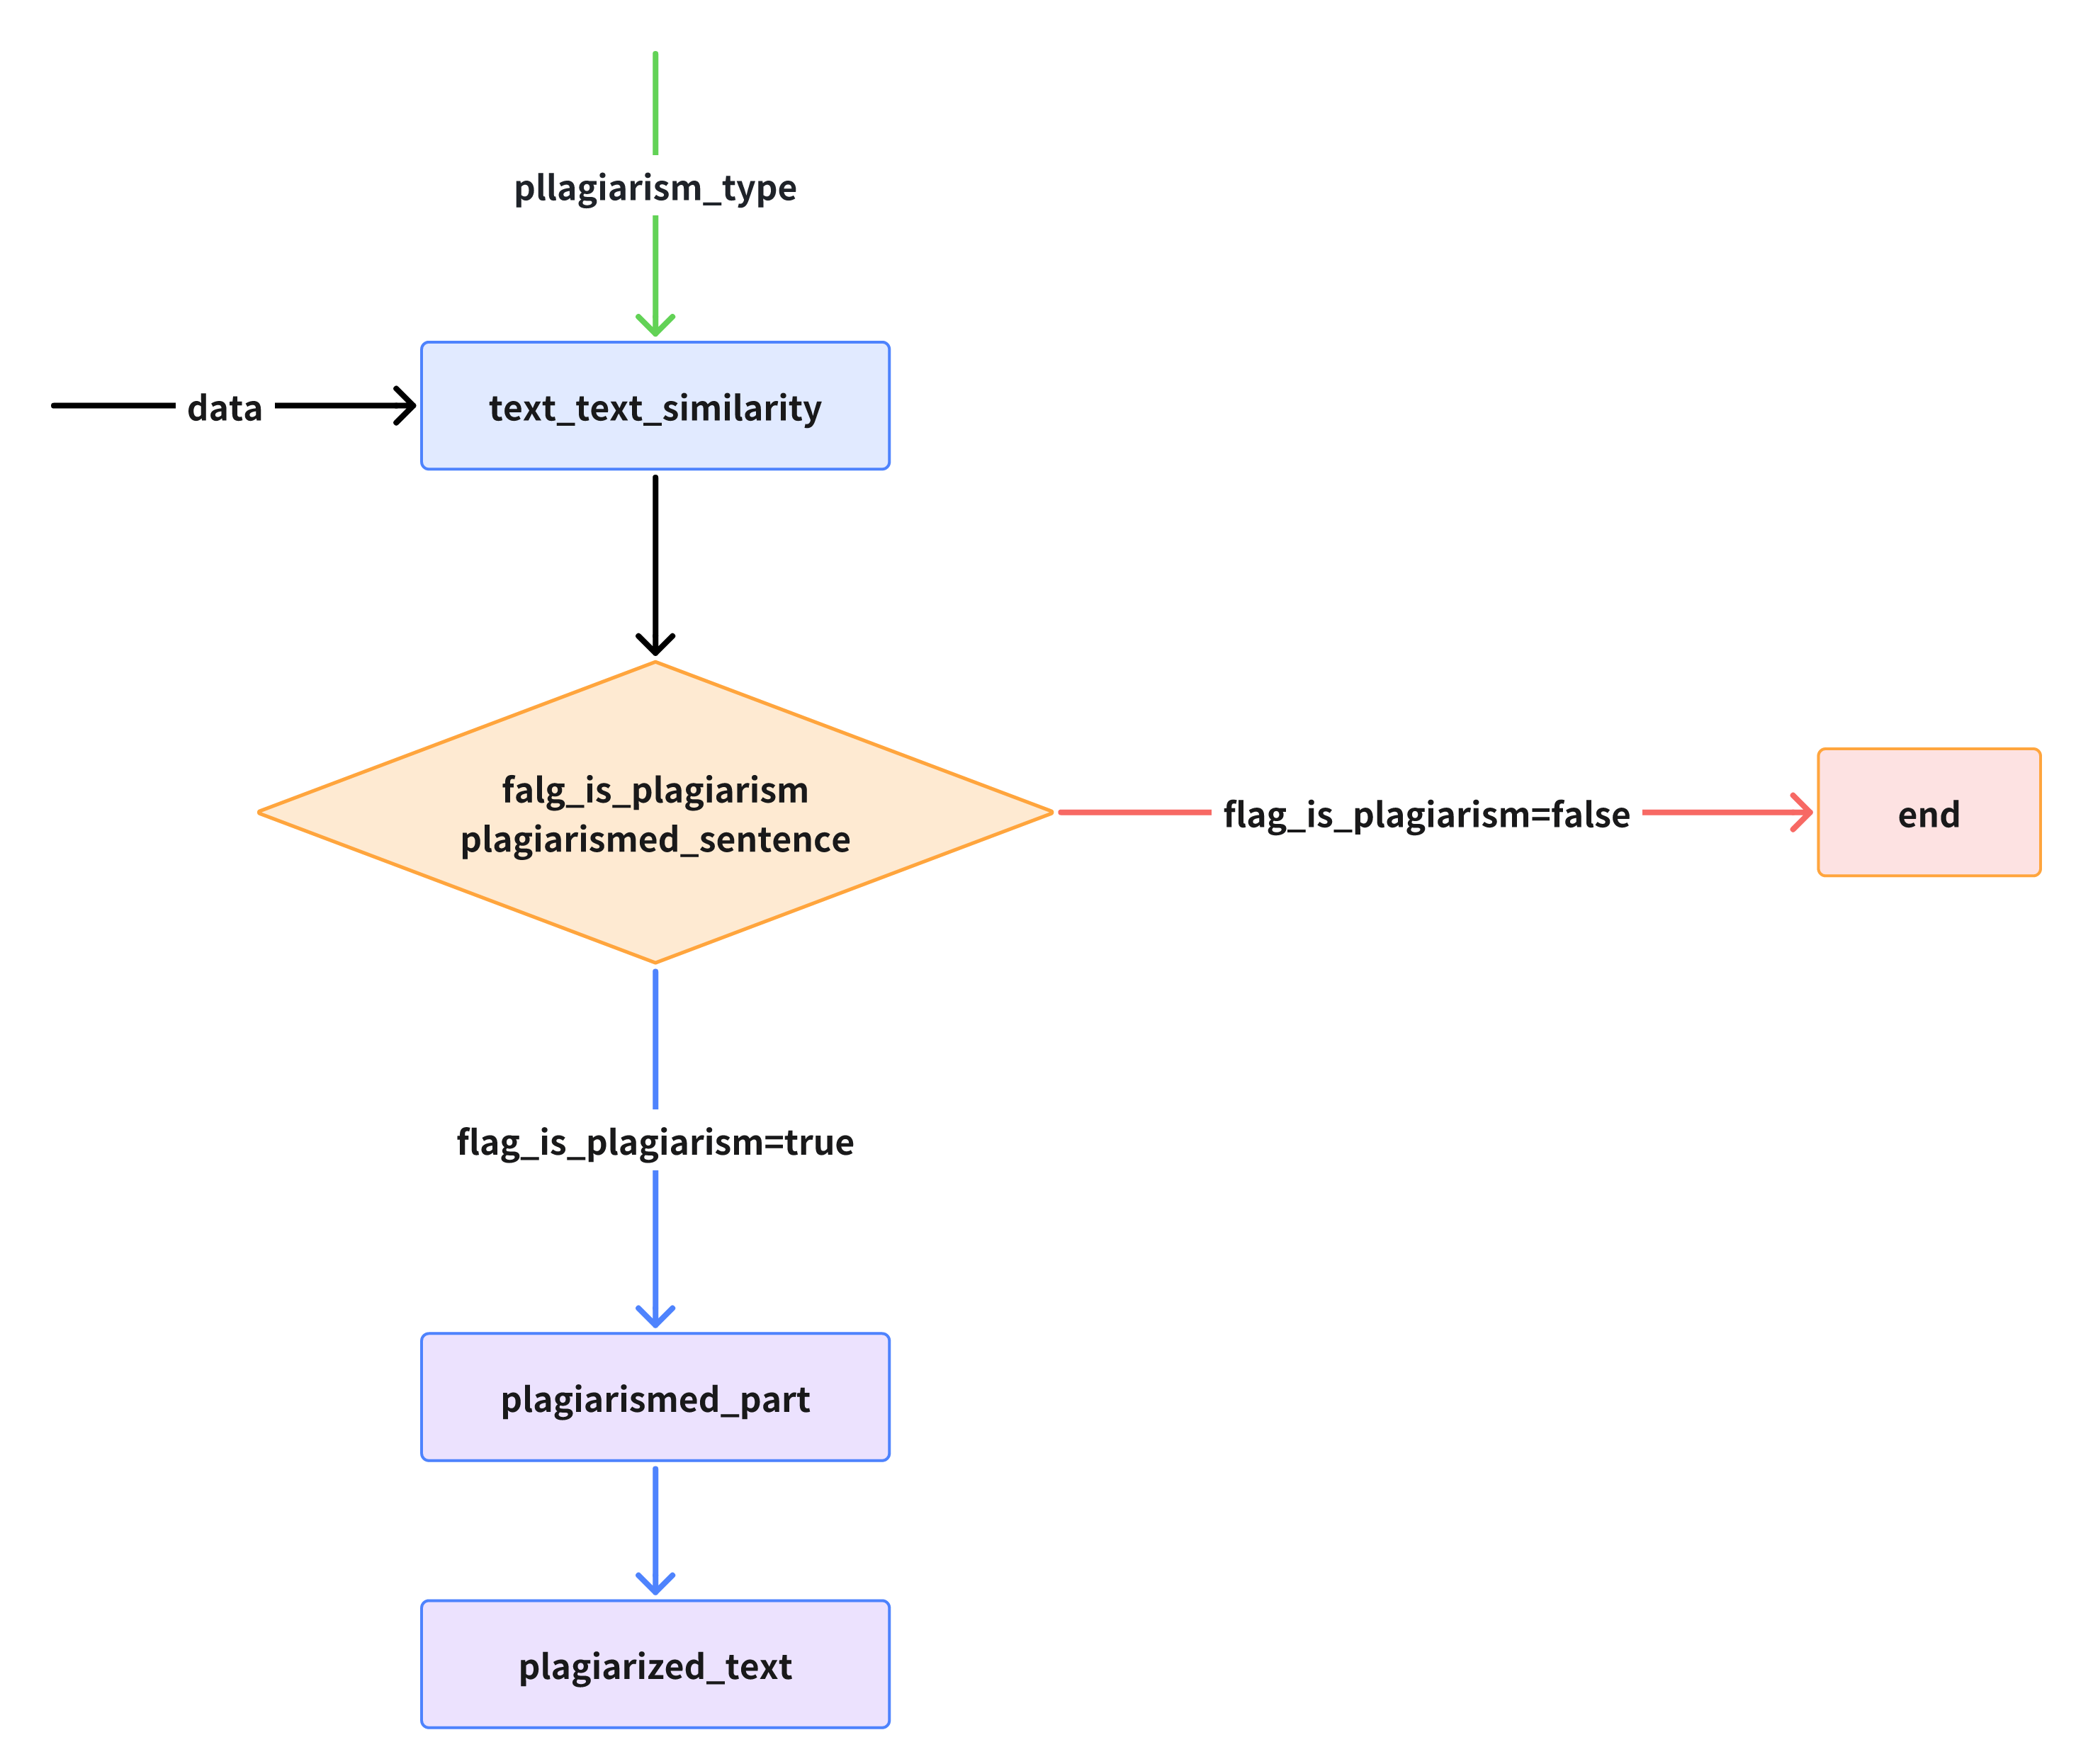
\includegraphics[width=1\linewidth]{png/system.png}
    \caption{system framework}
    \label{fig:2}
\end{figure}

Below are the steps for a simple experiment, where you can see the detailed process of how we conducted it.

\subsection{Input}
\textbf{Input}:QuerySentence = "I enjoy playing basketball with my friends. We play every weekend."

Our goal is to find the text most similar to this sentence in our corpus.

\subsection{Similarity Retrieval}
\

In this section, our goal is to retrieve the three text segments from the corpus that are most semantically similar to the query sentence. The core of this process lies in calculating the similarity between the query sentence and each text in the corpus, ranking them by similarity scores, and selecting the top three most relevant segments. Cosine similarity is used as the measure for similarity. Before computation, the texts are converted into vector embeddings using SentenceTransformer.

So now we get the ouput:
Most similar sentences:\\
1. He enjoy playing basketball with my friends. They play every weekend. (Similarity: 0.5823)\\
2. Friendship makes life more enjoyable. It adds meaning to our lives. (Similarity: 0.3458)\\
3. I am learning to play the guitar. It's a challenging but rewarding hobby. (Similarity: 0.3156)\\
Plagiarism has occurred\\
Query: I enjoy playing basketball with my friends. We play every weekend.\\
Most similar sentences: He enjoy playing basketball with my friends. They play every weekend.

\subsection{Get the most similar text}
\

In the previous section, we identified the most similar texts based on cosine similarity, and if the similarity exceeded 0.5, we considered the possibility of plagiarism. In this section, we attempt to more accurately identify the potential plagiarized parts.

Specifically, we first split all the texts into individual sentences. Next, we divide the text data into two categories: the original text dataset and the plagiarized text dataset. For each sentence in the plagiarized dataset, we compare it with every sentence in the original text dataset, calculate their similarities, and find the most similar sentence. Through this method, we can not only identify the similarity between two sentences but also precisely locate the parts where plagiarism is most likely involved.

\textbf{Ouput}:\\
The most likely plagiarized text is:\\
We play every weekend.\\
They play every weekend.\\
Their similarity is: 0.8143205
\section{Discussion}

In this experiment, our main goal was to distinguish between three types of cases: non-plagiarism, explicit plagiarism, and implicit plagiarism. However, during the implementation process, our experimental approach had certain limitations and shortcomings. First, using cosine similarity as the criterion for similarity detection, although it can measure the similarity between texts to some extent, also has obvious flaws. The calculation of cosine similarity is based on the vector space model, which primarily focuses on the directional similarity of text vectors while ignoring the specific positional relationships of words and phrases in the text. Therefore, for implicit plagiarism—especially in cases where the sentence order is rearranged to avoid detection—cosine similarity performs poorly. In some cases, even if the sentence order changes, as long as the arrangement of words and the overall meaning don't change significantly, cosine similarity may fail to effectively detect plagiarism.

In addition, our threshold for similarity had some arbitrary aspects. We used a fixed threshold of 0.5 to judge whether plagiarism occurred, but this value may not be optimal. It is possible that a threshold other than 0.5 could more accurately reflect the criteria for detecting plagiarism, but we did not conduct in-depth research or experimental verification on this matter. If we had tested and optimized various thresholds systematically, we might have achieved more convincing results in identifying plagiarism.

Overall, due to time constraints, the design and implementation of this experiment were rushed, leading to many shortcomings. For example, we did not conduct thorough experimental exploration in areas such as text preprocessing, model selection, and parameter adjustment, nor did we compare the effectiveness of different methods. Additionally, the scale and diversity of the experimental samples were not fully considered, which may have caused biases in the results and incomplete conclusions. Therefore, for future research in similar areas, we will need more time and resources to conduct systematic optimization and verification in order to improve the accuracy and robustness of the experimental methods.
\section{summarize}

In this experiment, our main objective was to distinguish between non-plagiarism, explicit plagiarism, and implicit plagiarism by calculating the similarity between texts. The entire experimental process can be divided into the following key steps:

\begin{enumerate}
    \item \textbf{Data Preparation}: We first collected and organized the relevant text data, which includes three types of texts: non-plagiarized, explicitly plagiarized, and implicitly plagiarized. We used GPT to assist in generating data, and in addition, we manually generated some of the data.
    
    \item \textbf{Text Vectorization}: In order to compute the similarity between texts, we used the \texttt{SentenceTransformer} model to convert the texts into vector embeddings. This step is crucial for the experiment because only by converting the text into numerical vectors can we perform the subsequent similarity calculations.
    
    \item \textbf{Similarity Calculation}: We used cosine similarity as the measure of text similarity. By calculating the cosine similarity between the query sentence and each sentence in the corpus, we were able to identify the most similar sentences and determine whether plagiarism exists. For each pair of sentences, we calculated their cosine similarity and selected the most similar sentence for further analysis.
    
    \item \textbf{Plagiarism Localization}: To identify the most likely plagiarized sections, we split the texts into independent sentences and compared each sentence from the plagiarized dataset with every sentence in the original dataset. This way, we could detect plagiarism even if the sentence order was changed, as long as the content of the text remained similar.
    
    \item \textbf{Threshold Setting and Judgment}: We set a fixed similarity threshold (0.5), and when the similarity exceeded this threshold, we considered the texts to be possibly plagiarized. However, this threshold choice may not be optimal, and in the future, it can be adjusted and optimized to improve the accuracy of the judgment.
    
    \item \textbf{Experiment Analysis and Conclusion}: Through the experiment, we identified several potential plagiarized texts. The system performed well in detecting explicit plagiarism, but there were certain limitations in detecting implicit plagiarism, especially when the sentence order was changed. The similarity calculation might not fully reveal plagiarism behavior in such cases.
\end{enumerate}

Overall, while this experiment achieved certain goals, there were limitations due to time and resource constraints, particularly in detecting implicit plagiarism and setting the similarity threshold. Future research can improve plagiarism detection accuracy and robustness by incorporating more semantic information, optimizing models, and adjusting thresholds.

\section{Team Contribution}
\

Our team division of labour and contribution is follow:
\begin{itemize}
    \item \textbf{Zhang Sibo}: Model construction and training, paper writing, project management, 40\% 
    \item \textbf{Ye Debo}: Paper writing, data collection, 20\%
    \item \textbf{Zou Yifan}: Data collection, data processing and testing, 20\%
    \item \textbf{Li Yonghui}: Data collection, data processing and testing, 20\%
\end{itemize}


\section{Appendix}

\subsection{Instruction}

\subsubsection{innovation point}
\begin{itemize}
    \item Multiple self-collected datasets -- 40\% Innovation
    \item Effective fine-tuning of existing models -- 30\% Innovation
\end{itemize}

\subsubsection{Source of Code}
\

Our code is partially based on this video~\cite{video}, which provided us with some ideas and a framework for implementation. However, we did not directly copy the code from the video; instead, we modified and optimized it according to our own requirements. The majority of the code was written by ourselves, especially in the plagiarism detection part, where we designed and implemented independent functional modules to ensure the customizability and flexibility of the entire experiment. During the development process, we not only borrowed some implementation methods from the video but also conducted extensive trials and testing to ensure the effectiveness and reliability of the code.

\subsubsection{Innovation motivation and problem that needs to be solved}
\

Innovative motivation: Solving the problem of plagiarism localization that cannot be achieved by traditional text similarity retrieval methods.

\subsubsection{Comparison of improvements with reference papers}
\

We used the FAISS library provided in the reference paper and did not make other innovations in text recognition. Our main contribution lies in text plagiarism localization detection, so the level of improvement compared to the reference paper cannot be measured.

\subsection{The process of generating data}
\subsubsection{Non-plagiarism}
\textbf{Q:} Suppose you are an original author, and reading other people's words inspires you. Example:  \\
\textbf{Original sentence}: She spent the afternoon reading a new chapter, eager to understand the concepts and apply them in practice.  \\
\textbf{Generated sentence}: After attending the workshop, he felt more confident in using the new software to complete his assignments.  

We can see that while both sentences describe something related to learning, we can tell that they are on the same topic rather than being plagiarized. This is because, despite both sentences involving the process of learning and understanding, they present different aspects of learning through different contexts, time points, and tasks, which is enough to confirm that these sentences are not plagiarized.

To explain further, we can understand that within the same theme, authors can convey information in different ways, leading to many different expressions under the same theme. Each of these ways represents a new description of the theme. For instance, in the original sentence, ``reading a new chapter" focuses on the active process of acquiring knowledge, while the generated sentence's ``attending a workshop" emphasizes learning through interactive software, showcasing two different but complementary ways of learning.

Now, based on this idea, expand it to multiple different themes, including learning, economics, environment, food, animals, politics, holidays, wellness, tourism, history, etc. Each theme should present sentences with different details, contexts, or actions, focusing on their specific aspects, ensuring sentences revolve around the same theme but differ in their expression, thus avoiding plagiarism.\\

\\\\\\\\

\textbf{Q}: Suppose you need to generate a series of sentences for a diverse theme library, covering various fields such as learning, economy, environment, animals, politics, tourism, science fiction, literature, mythology, traditional Chinese medicine, movies, artificial intelligence, etc. When generating sentences for these themes, please consider the following requirements:  \\
1. Each sentence should be closely related to the theme and accurately reflect the core content or key viewpoints of that theme.  \\
2. The sentences should be creative, expressing unique viewpoints or descriptions. Simple copying and pasting of existing ideas or texts is prohibited. Avoid excessive similarity between the original sentence and others, even within the same theme, ensuring the uniqueness of each sentence.  \\
3. The format of the sentences can be diverse. They can express a viewpoint, analyze a phenomenon, describe a scene, raise a question, or predict a trend, etc.  \\
4. Each sentence should focus on specific details, highlighting the theme's emphasis, and convey different ideas and meanings.  

Please generate a corpus based on these requirements and ensure that each sentence is unique.\\

\\
\textbf{Q}: You need to generate sentences that contain explicit plagiarism based on the original sentence. Common methods for explicit plagiarism include replacing keywords, rearranging sentence structure, changing modifiers or parts of phrases, etc. This approach generally keeps the overall structure and core meaning of the sentence unchanged, only modifying certain parts to make it appear different from the original sentence. For example, by replacing keywords:

\textbf{Original sentence}:  
The sun sets in the west, painting the sky with hues of orange and red.  

\textbf{Explicit plagiarism sentence}:  
The sun descends in the west, coloring the sky with shades of orange and crimson.

\subsubsection{Implicit plagiarism}
\textbf{Q}: Implicit plagiarism refers to the use of someone else's ideas, viewpoints, structure, or expression without directly citing their work, resulting in content that is somewhat similar to the original.\\
\textbf{For example}:  \\
\textbf{Original}: "The cat sat on the mat. It looked very comfortable." \\
\textbf{Plagiarized}: "On the mat, the cat sat. It appeared quite comfortable."

\subsubsection{Explicit plagiarism}
\textbf{Q}: Suppose you are an original author. By learning from other people's writings, you can gain more creative inspiration, but that does not constitute explicit plagiarism.\\
\textbf{Example}:\\
\textbf{Original sentence}: The cat sat on the mat. It looked very comfortable.\\
\textbf{Plagiarized sentence}: The dog lay on the rug. It seemed very relaxed.

It can be observed that these two sentences describe a similar scene—an animal in a resting state. However, the difference lies merely in the replacement of keywords (such as changing "cat" to "dog" and "mat" to "rug"), while the sentence structure and core information remain nearly identical. This kind of writing, where only a few words or phrases are replaced, constitutes explicit plagiarism. In other words, explicit plagiarism typically retains the original sentence's grammatical framework and core description, only disguising the "difference" by changing some nouns, verbs, or adjectives, without making substantial changes to the sentence's main idea, context, or information. For example, in the original sentence, "The cat sat on the mat" describes the scene of "the cat resting on a mat," while the plagiarized sentence simply replaces keywords, still describing "an animal resting on some object." This does not possess enough originality.

Under different themes, explicit plagiarism will also follow a similar pattern: only surface-level vocabulary is modified, without presenting new contexts, details, or perspectives. This way of creation not only violates the principle of originality but also fails to reflect the author's deep understanding of the theme.\\

Now, I need you to generate a dataset for implicit plagiarism. The dataset should contain both the original and plagiarized sentences, each containing more than 80 characters. 

Output format:  
"The children played outside until it got."  
"Until it got dark, the children played outside."

Please output in a code block format.
\\\\
\textbf{Q}: Based on the data you have generated, the following new requirements are proposed: \\ 
1. Each sentence in the dataset should contain implicit plagiarism.  \\
2. Expand the methods of implicit plagiarism in each group, so that each sentence may have different ways of plagiarism (e.g., word order adjustment, passive voice change, phrase rephrasing, etc.).  \\
3. The dataset should cover a variety of scenarios, with sentences describing everyday activities, emotional expressions, and other diverse themes.  \\
4. Generate as much data as possible and output it in a code block format.
% 引用:
{
    \small
    \bibliographystyle{ieeenat_fullname}
    \bibliography{main}
}

% WARNING: do not forget to delete the supplementary pages from your submission 
% \clearpage
% \setcounter{page}{1}
% \maketitlesupplementary


% \section{Rationale}
% \label{sec:rationale}
% % 
% Having the supplementary compiled together with the main paper means that:
% % 
% \begin{itemize}
% \item The supplementary can back-reference sections of the main paper, for example, we can refer to \cref{sec:intro};
% \item The main paper can forward reference sub-sections within the supplementary explicitly (e.g. referring to a particular experiment); 
% \item When submitted to arXiv, the supplementary will already included at the end of the paper.
% \end{itemize}
% % 
% To split the supplementary pages from the main paper, you can use \href{https://support.apple.com/en-ca/guide/preview/prvw11793/mac#:~:text=Delete%20a%20page%20from%20a,or%20choose%20Edit%20%3E%20Delete).}{Preview (on macOS)}, \href{https://www.adobe.com/acrobat/how-to/delete-pages-from-pdf.html#:~:text=Choose%20%E2%80%9CTools%E2%80%9D%20%3E%20%E2%80%9COrganize,or%20pages%20from%20the%20file.}{Adobe Acrobat} (on all OSs), as well as \href{https://superuser.com/questions/517986/is-it-possible-to-delete-some-pages-of-a-pdf-document}{command line tools}.

\end{document}
